\chapter{Desenvolvimento de Projetos com o AndroMDA}

Nesta seção veremos os passos necessários ao desenvolvimento de projetos com o MDArte, utilizando os cartuchos EJB, Hibernate e BPM4Struts.

\section{Criação de um Novo Projeto e Configuração do ambiente}

O plugin do MDArte para o Maven já possui um procedimento parametrizado para criação de projetos, que funciona como um wizard, onde o usuário deve responder a perguntas. Através das respostas fornecidas, o MDArte direcionará a criação da estrutura básica e dos artefatos básicos de configuração de projetos. O procedimento para criação de um novo projeto é:

\begin{enumerate}
\item Abra o terminal (command prompt) e vá para o diretório onde se deseja
criar o projeto. Na verdade, o projeto será gerado em um subdiretório do diretório escolhido. No Windows, não
se pode ter espaços em branco no caminho desse diretório. Exemplo de diretório inválido:
C:$\backslash$Documents and Settings$\backslash$MDArte.

\item Digite o comando: maven andromdapp:generate

\item Responda as perguntas de acordo com o seu projeto. Abaixo um exemplo com
respostas típicas (perguntas em negrito):

\textbf{Please enter your first and last name (i.e. Rodrigo Salvador):} \\
MDArte\\
\textbf{Please enter the name of your J2EE project (i.e. Sistema Academico):}\\
Sistema Academico\\
\textbf{Please enter the id for your J2EE project (i.e. sistemaacademico):}\\
sistemaacademico\\
\textbf{Please enter a version for your project (i.e. 1.0):}\\
1.0\\
\textbf{Please enter the base package name for your J2EE project (i.e.
br.mdarte.exemplo.academico):}\\
br.mdarte.exemplo.academico\\
\textbf{Would you like to enable security? (enter 'yes' or 'no')?}\\
yes\\
\textbf{Would you like to use oAuth (enter 'yes' or 'no') ?}\\
no\\
\textbf{Would you like to use MDArte's default Controle Acesso (enter 'yes' or
'no') ?}\\
yes\\
\textbf{Would you like to use modules (enter 'yes' or 'no')?}\\
yes\\
\textbf{Please enter the EJB version number (enter '2' or '3'):}\\
3\\
\textbf{Please enter the Struts version number (enter '1' or '2'):}\\
2\\
\textbf{Would you like to enable the JUnit support for general testing? (enter
'yes' or 'no')? }\\
 no\\
\textbf{Please enter the database backend for the persistence layer: (enter
'hypersonic' or 'mysql' or 'oracle' or 'postgres')}\\
 postgres\\
 
\item Após receber as respostas, o MDArte criará um subdiretório onde será
 gerada a estrutura inicial do projeto. A partir desse momento chamaremos esse diretório de <DiretorioProjeto>.

\item Ainda no console, vá para o diretório onde está seu projeto:
<DiretorioProjeto>.

\item Digite maven. Isto obrigará o Maven a obter todos os artefatos (por
exemplo, bibliotecas) de que o projeto dependerá.

\end{enumerate}

\section{Configuração do Banco}
Para se configurar o Banco de Dados é necessário modificar o arquivo project.properties
da raiz do projeto, onde se encontram as propriedades que devem ser alteradas. Abaixo estão as
propriedades do arquivo de configuração para cada um dos Bancos de Dados

\begin{itemize}
	\item [Oracle] \hfill
		\begin{itemize}
			\item
			dataSource.driver.jar=\textdollar{}\{env.JBOSS\_HOME\}/server/default/lib/hsqldb.jar
			\item dataSource.driver.class=oracle.jdbc.driver.OracleDriver
			\item sql.mappings=Oracle9i
			\item hibernate.db.dialect=org.hibernate.dialect.Oracle9Dialect
		\end{itemize}
	\item [SQLServer] \hfill
		\begin{itemize}
			\item
			dataSource.driver.jar=\textdollar{}\{env.JBOSS\_HOME\}/server/default/lib/hsqldb.jar
			\item dataSource.driver.class=oracle.jdbc.driver.OracleDriver
			\item sql.mappings=Oracle9i
			\item hibernate.db.dialect=org.hibernate.dialect.Oracle9Dialect
		\end{itemize} 
	\item [Postgres] \hfill
  		\begin{itemize}
			\item
			dataSource.driver.jar=\textdollar{}\{env.JBOSS\_HOME\}/server/default/lib/hsqldb.jar
			\item dataSource.driver.class=oracle.jdbc.driver.OracleDriver
			\item sql.mappings=Oracle9i
			\item hibernate.db.dialect=org.hibernate.dialect.Oracle9Dialect
		\end{itemize}
	\item [MySQL] \hfill
		\begin{itemize}
			\item
			dataSource.driver.jar=\textdollar{}\{env.JBOSS\_HOME\}/server/default/lib/hsqldb.jar
			\item dataSource.driver.class=oracle.jdbc.driver.OracleDriver
			\item sql.mappings=Oracle9i
			\item hibernate.db.dialect=org.hibernate.dialect.Oracle9Dialect
		\end{itemize}
\end{itemize}

Outro arquivo que deve ser alterado ou criado é o arquivo de configurações do Banco de
Dados do JBoss, localizado no diretório JBOSS\_HOME/server/default/deploy/, com
formação do nome terminando com -ds.xml (ex.: aplicacoes-ds.xml), que deve ter a tag <local-tx-datasource> preenchida de acordo com as informações fornecidas no arquivo <projeto>/project.properties.
Exemplo (usando banco Postgres):

\begin{lstlisting}[language=xml]
<local-tx-datasource>
	<jndi-name>sistemaacademicoDS</jndi-name>
	<use-java-context>true</use-java-context>
	<connection-url>jdbc:postgresql://127.0.0.1:5432/sistemaacademico</connection-url> 
	<driver-class>org.postgresql.Driver</driver-class>
		<user-name>usuario</user-name>
		<password>senha</password>
	<!--<exception-sorter-class-name>org.jboss.resource.adapter.jdbc.vendor.OracleExceptionSorter</exception-sorter-class-name>-->
</local-tx-datasource>
\end{lstlisting}

Repare que no exemplo anterior, o nome do Data Source é sistemaacademicoDS, que
deve ser o mesmo nome informado no arquivo project.properties da raiz do projetom ou
seja `sistemaacademicoDS`.

Além disso, é necessário alterar o arquivo login-config.xml, localizado no
diretório JBOSS\_HOME/server/default/conf/, deverá ser modificado, adicionando o
seguinte trecho:

\begin{lstlisting}[language=xml]
<!--
SistemaAcademico Policy
-->
<application-policy name="sistemaacademico">
	<authentication>
		<login-module code="org.jboss.security.ClientLoginModule"
			flag="required">
			<module-option name="multi-threaded">true
				</module-option>
		</login-module>
		<login-module code="accessControl.LoginModuleImpl" 
			flag="required">
			<module-option name="dsJndiName">java:/controleacessoDS
				</module-option>
			<module-option name="unauthenticatedIdentity">guest
				</module-option>
			<module-option name="principalClass">
				accessControl.PrincipalImpl</module-option> 
			<module-option name="hashEncoding">hex</module-option> 
			<module-option name="hashAlgorithm">md5</module-option>
			<module-option name="principalsQuery">
				select SENHA from OP_C_A where LOGIN=?
				</module-option>
			<module-option name="rolesQuery">
				select OP_PF.PF_OP_C_A_FK, 'Roles'
				12from OP_C_A, OP_C_A_PF_OP_C_A OP_PF
				where LOGIN=? AND OP_C_A.ID = OP_PF.OP_C_A_FK
			</module-option>
		</login-module>
	</authentication>
</application-policy>
\end{lstlisting}

As informações presentem nesse arquivo permitirão a aplicação do Sistema Acadêmico se
conectar a base de dados e validar o usuário no momento de login.

\section{Controle de Acesso}

Neste tutorial estaremos utilizando funcionalidades de controle de acesso, porém não é
nosso propósito explorar suas funcionalidades. Assim, estaremos utilizando um projeto de controle
de acesso desenvolvido pela comunidade do MDArte.
O projeto pode ser obtido a partir do repositório Git do MDArte,
pelo endereço https://github.com/MDArte/controleacesso.git . Por fim, edite também o
arquivo project.properties do ControleAcesso para configurar o tipo de Banco de Dados a ser
utilziado, conforme realizado com o projeto SistemaAcademico. Note que a propriedade
dataSource.name está definida como ControleAcessoDS.
Novamente, precisaremos criar um arquivo de configuração do Banco de Dados, localizado
no diretório JBOSS\_HOME/server/default/deploy/ . O nome do arquivo deve seguir
a mesma formatação mencionada, terminando em -ds.xml (ex.: aplicacoes-ds.xml), podendo estar no mesmo
arquivo com as configurações do projeto SistemaAcademico.

Exemplo:

\begin{lstlisting}[language=xml]
<local-tx-datasource>
	<jndi-name>controleacessoDS</jndi-name>
	<use-java-context>true</use-java-context>
	<connection-url>jdbc:postgresql://127.0.0.1:5432/controleacesso
		</connection-url> 
	<driver-class>org.postgresql.Driver</driver-class>
	<user-name>usuario</user-name>
	<password>senha</password>
	<!--<exception-sorter-class-name>
		org.jboss.resource.adapter.jdbc.vendor.OracleExceptionSorter
		</exception-sorter-class-name>-->
</local-tx-datasource>
\end{lstlisting}

Note que no exemplo anterior o ControleAcesso estará utilizando a mesma base de dados
do projeto SistemaAcademico, definida pela tag <connection-url>. Agora, execute os seguinte
comandos, na raiz do projeto ControleAcesso, para gerar, compilar e copiar os pacotes para o
diretório JBOSS\_HOME/server/default/deploy/:

\begin{lstlisting}[language=bash]
maven mda -Dprojeto=ca-core
cd common
maven jar:install deploy
cd ../core/cd
maven jar:install deploy
\end{lstlisting}

\section{Modelando o nosso primeiro projeto}

Nesta seção iremos modelar um exemplo de Sistema Acadêmico básico, mostrando o
quão rápido e simples pode ser usar o MDArte e todo o seu poder de geração.

Para esta parte do tutorial usaremos o MagicDraw. Na barra de ferramentas do
MagicDraw, clicaremos em 'Open Project' e abriremos o xml do projeto,
SistemaAcademico.xml no caminho
<Diretório-do-Projeto>/mda/src/uml/.

\subsection{Modelando a camada de domínio}
Na camada de domínio, estarão as classes do domínio da aplicação. Elas serão entidades e
estarão associadas a algum modo de persistência. Essas classes deverão conter o estereótipo
«Entity» e os atributos que serão persistidos. Todas as classes de entidade devem obrigatoriamente
estar no pacote <PacoteProjeto>.cd, em que <PacoteProjeto> é o pacote definido para o projeto.
Atualmente, estamos utilizando framework Hibernate para esta camada. 

Neste exemplo, especificamente, iremos também marcar nossas entidades com o
estereótipo «Manageable», tal marcação diz para o MDArte que desejamos que seja
gerado um CRUD padrão para tais entidades, sem a necessidade de modelarmos o
mesmo diretamente.

\begin{enumerate}
	\item Crie a mesma estrutura de pacotes que foi definida na criação do projeto.
Dentro da estrutura, crie o pacote “cd”.
		\begin{figure}[!htb]
			\centering
			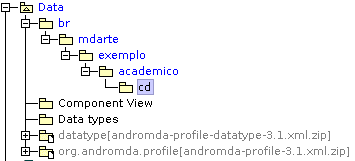
\includegraphics[width=250pt,height=100pt]{imgs/tutorial-mdarte-0000.png}
		\end{figure}
	\item Clique com o botão direito do mouse no pacote “cd” e selecione a opção New Diagram .
Em seguida, selecione Class Diagram.
		
		\begin{figure}[!htb]
			\centering
			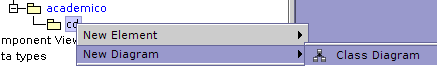
\includegraphics[width=400pt,height=60pt]{imgs/tutorial-mdarte-0001.png}
		\end{figure}
	
	\item Indique o nome desejado para diagrama (ex: Entidades).
	
	\item No diagrama de classe, crie uma nova classe. Clique com o botão direto
	sobre a classe e selecione a opção Specification. Defina o nome da classe como “Estudante”.
	
	\item Crie os atributos na classe Estudante (matricula, nome) selecionando a aba Attributes e
clicando no botão Add. A figura abaixo exemplifica a criação do atributo matricula. O
campo Visibility deve ser public. Não é necessário modelar o atributo id, pois
ele é gerado automaticamente.

		\begin{figure}[!htb]
			\centering
			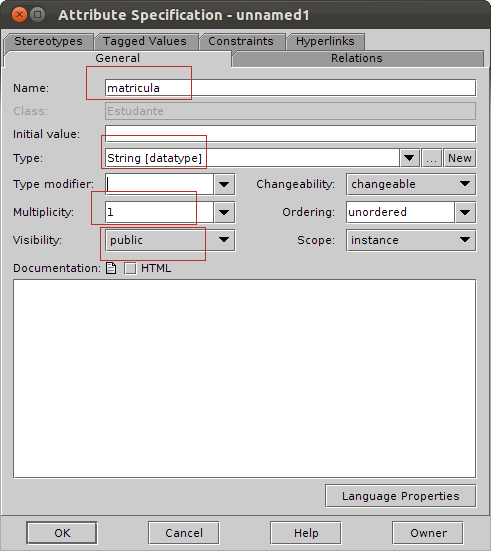
\includegraphics[width=350pt,height=400pt]{imgs/tutorial-mdarte-0002.png}
		\end{figure}
		
	A multiplicidade com valor 1 (campo Multiplicity) indica que o atributo é obrigatório (NOT
NULL), já o valor 0..1 indica que o atributo não é obrigatório. Por padrão, todos os atributos são
gerados como NOT NULL.
\end{enumerate}